\appendix
\chapter{Abbildungen}\label{appen}
\phantom{Platzhalter}
\begin{figure}[H]\leavevmode
    \centering
    \resizebox{0.85\textwidth}{!}{ 
    \begin{minipage}{\textwidth}
    \captionsetup[subfigure]{justification=centering}
    \begin{subfigure}{\textwidth}
        \centering
        \caption{\(n=2\)}
        \begin{tabular}{lrrrrr}
            \toprule
            & \multicolumn{2}{c}{Merkmale} \\
            \cmidrule(lr){2-3}
            Objekte & A & B \\ 
            \midrule
            \(O_1\)  & 1,3 & -0,4  \\
            \(O_2\) & -1,6 & 2,1 \\
            \(O_3\) & 1,2 & 0,7 \\
            \(O_4\) & -2,1 & 0,6 \\
            \(O_5\) & 0,8 & 0,6 \\
            \(O_6\) & -0,3 & 1,6 \\
            \bottomrule
        \end{tabular}
        \hspace{35pt}
        \begin{tikzpicture}[baseline=(current bounding box.center)]
            \begin{axis}[
                xlabel={A},
                ylabel={B},
                width=0.45\textwidth,
                anchor=center,
            ]
            \addplot[only marks,mark options={fill=blue, color=blue}] coordinates {
                (1.3,-0.4) 
                (-1.6,2.1)
                (1.2,0.7)
                (-2.1,0.6)
                (0.8,0.6)
                (-0.3,1.6)
            };
            \end{axis}
        \end{tikzpicture}
    \end{subfigure}
    \begin{subfigure}{\textwidth}
        \centering
        \caption{\(n=3\)}
        \begin{tabular}{lrrrrr}
            \toprule
            & \multicolumn{3}{c}{Merkmale} \\
            \cmidrule(lr){2-4}
            Objekte & A & B & C \\ 
            \midrule
            \(O_1\)  & 1,3 & -0,4 & 1,9 \\
            \(O_2\) & -1,6 & 2,1 & 0,2 \\
            \(O_3\) & 1,2 & 0,7 & 0,4 \\
            \(O_4\) & -2,1 & 0,6 & -0,2 \\
            \(O_5\) & 0,8 & 0,6 & 1,1 \\
            \(O_6\) & -0,3 & 1,6 & 0.8 \\
            \bottomrule
        \end{tabular}
        \hspace{17pt}
        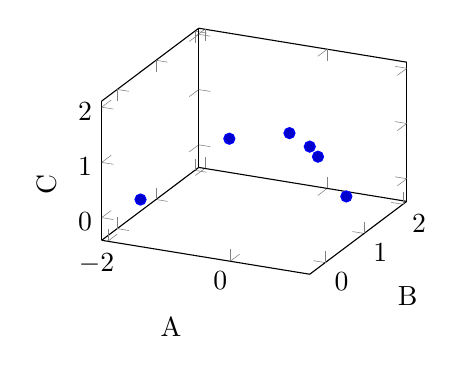
\begin{tikzpicture}[baseline=(current bounding box.center)]
            \begin{axis}[
                xlabel={A},
                ylabel={B},
                zlabel={C},
                width=0.45\textwidth,
                anchor=center,
            ]
            \addplot3+[only marks] coordinates {
                (1.3,-0.4,1.9) 
                (-1.6,2.1,0.2)
                (1.2,0.7,0.4)
                (-2.1,0.6,-0.2)
                (0.8,0.6,1.1)
                (-0.3,1.6,0.8)
            };
            \end{axis}
        \end{tikzpicture}
    \end{subfigure}
    \begin{subfigure}{\textwidth}
        \caption{\(n=4\)}
        \begin{tabular}{lrrrrrr}
            \toprule
            & \multicolumn{4}{c}{Merkmale} \\
            \cmidrule(lr){2-5}
            Objekte & A & B & C & D \\ 
            \midrule
            \(O_1\)  & 1,3 & -0,4 & 1,9 & 0.7 \\
            \(O_2\) & -1,6 & 2,1 & 0,2 & 0.9 \\
            \(O_3\) & 1,2 & 0,7 & 0,4 & 1.3 \\
            \(O_4\) & -2,1 & 0,6 & -0,2 & 0.5 \\
            \(O_5\) & 0,8 & 0,6 & 1,1 & -0.8 \\
            \(O_6\) & -0,3 & 1,6 & 0.8 & -1.3 \\
            \bottomrule
        \end{tabular}
        \hspace{45pt}
        
\begin{tikzpicture}[baseline=(current bounding box.center)]
            \draw[thick] (-2,-2) rectangle (2,2);
            \node at (0,0) {\Huge \textbf{?}};
        \end{tikzpicture}
    \end{subfigure}
    \end{minipage}
    }
    \caption{Plotten von Daten in verschiedenen Dimensionen}\label{fig:pcadim}
\end{figure}
